\documentclass[11pt,letterpaper]{article}

% bioRxiv-style packages
\usepackage[utf8]{inputenc}
\usepackage[T1]{fontenc}
\usepackage{lmodern}
\usepackage[margin=1in]{geometry}
\usepackage{graphicx}
\usepackage{amsmath,amssymb,amsfonts}
% Chemical structures described textually
\usepackage{siunitx}
\usepackage{booktabs}
\usepackage{longtable}
\usepackage{array}
\usepackage{multirow}
\usepackage{float}
\usepackage{caption}
\usepackage{subcaption}
\usepackage[colorlinks=true,linkcolor=blue,citecolor=blue,urlcolor=blue]{hyperref}
\usepackage{natbib}
\usepackage{authblk}
% \usepackage{lineno}  % Line numbers disabled
\usepackage{setspace}
\usepackage{xcolor}
\usepackage{tikz}
\usetikzlibrary{shapes,arrows,positioning,calc}
\usepackage{enumitem}
\usepackage{fancyhdr}
\usepackage{lastpage}

% Page style
\pagestyle{fancy}
\fancyhf{}
\renewcommand{\headrulewidth}{0pt}
\fancyfoot[C]{\thepage}

% Line numbers disabled
% \linenumbers

% One-half spacing
\onehalfspacing

% Title formatting
\makeatletter
\renewcommand{\maketitle}{
\begin{center}
{\Large\bfseries\@title\par}
\vspace{1em}
{\normalsize\@author\par}
\vspace{1em}
{\small\@date\par}
\end{center}
}
\makeatother

% Custom commands
\newcommand{\IC}{\text{IC}_{50}}
\newcommand{\EC}{\text{EC}_{50}}
\newcommand{\Ki}{K_\text{i}}
\newcommand{\Kd}{K_\text{d}}

\title{Rational Design of Pathway-Selective Cannabinoid Compounds for Attention-Deficit/Hyperactivity Disorder: Dissociating Therapeutic Efficacy from Orexigenic Effects Through Biased Signaling, Prodrug Activation, and Multi-Target Pharmacology}

\author[1]{Matthew Long\thanks{Corresponding author: matthew@yonedaai.com}}
\author[2]{The YonedaAI Collaboration}
\affil[1]{Independent Researcher, Chicago, IL, USA}
\affil[2]{YonedaAI Research Collective}

\date{December 2024}

\begin{document}

\maketitle

\begin{abstract}
\noindent\textbf{Background:} The endocannabinoid system (ECS) modulates dopaminergic transmission in prefrontal-striatal circuits implicated in attention-deficit/hyperactivity disorder (ADHD). While cannabinoid receptor type 1 (CB1) activation shows theoretical potential for modulating executive function, therapeutic development is hindered by unwanted effects including appetite stimulation, psychoactivity, and cognitive impairment. The challenge of dissociating beneficial from detrimental CB1-mediated effects represents a significant medicinal chemistry problem.

\noindent\textbf{Objective:} To develop a comprehensive rational drug design framework for creating $\Delta^9$-tetrahydrocannabinol (THC) analogs that preserve ADHD-relevant prefrontal cortex modulation while eliminating orexigenic effects through mechanistically distinct strategies.

\noindent\textbf{Methods:} We integrated current understanding of CB1 receptor structural biology, biased signaling mechanisms, regional enzyme distribution, and appetite circuit pharmacology to design three complementary chemical strategies: (A) Gi-biased partial agonists and allosteric-orthosteric hybrids exploiting pathway-selective signaling; (B) prodrug approaches utilizing differential CYP450 and esterase expression for cortex-selective activation; and (C) multi-target ligands simultaneously engaging CB1 while antagonizing appetite-related receptors.

\noindent\textbf{Results:} We propose six lead compounds (YAC-101/102, YAC-201/202, YAC-301/302) with defined structural modifications, predicted pharmacological profiles, and synthesis considerations. Each compound class addresses specific mechanistic vulnerabilities in THC's pharmacology. We present a comprehensive preclinical validation framework including in vitro bias quantification, regional selectivity assessment, ADHD model behavioral testing, and appetite dissociation metrics.

\noindent\textbf{Conclusions:} This framework provides a systematic approach to cannabinoid drug design that may enable development of therapeutically useful CB1 modulators with improved side effect profiles. The strategies presented are broadly applicable to other therapeutic contexts where CB1 modulation shows promise but is limited by on-target toxicity.

\vspace{1em}
\noindent\textbf{Keywords:} cannabinoid, CB1 receptor, ADHD, biased signaling, prodrug, drug design, appetite, endocannabinoid system
\end{abstract}

\newpage

\section{Introduction}

\subsection{The Therapeutic Challenge of Cannabinoid Pharmacology}

The endocannabinoid system (ECS) represents one of the most ubiquitous neuromodulatory systems in the mammalian brain, with cannabinoid receptor type 1 (CB1) being the most abundant G protein-coupled receptor (GPCR) in the central nervous system \citep{herkenham1990cannabinoid}. The widespread distribution and diverse physiological functions of CB1 create both therapeutic opportunities and significant pharmacological challenges. While CB1 activation modulates numerous processes relevant to neuropsychiatric disorders—including attention, impulsivity, emotional regulation, and reward processing—the same receptor also mediates appetite stimulation, psychoactive effects, cognitive impairment, and dependence liability \citep{lu2016endocannabinoid}.

$\Delta^9$-Tetrahydrocannabinol (THC), the primary psychoactive constituent of \textit{Cannabis sativa}, exemplifies this challenge. Despite self-reported benefits for attention and focus in some individuals with attention-deficit/hyperactivity disorder (ADHD) \citep{mitchell2016cannabis}, THC's clinical utility is fundamentally limited by its pleiotropic central effects. The core question driving this research is whether modern understanding of GPCR pharmacology, particularly biased signaling and structural biology, can enable rational design of cannabinoid compounds that dissociate therapeutic from unwanted effects.

\subsection{ADHD and the Endocannabinoid System}

ADHD is characterized by developmentally inappropriate levels of inattention, hyperactivity, and impulsivity, affecting approximately 5\% of children and 2.5\% of adults worldwide \citep{faraone2015attention}. The neurobiological basis involves dysfunction in dopaminergic and noradrenergic transmission within prefrontal-striatal circuits, with first-line pharmacotherapies (stimulants, atomoxetine) acting primarily through catecholamine modulation \citep{arnsten2009toward}.

The ECS intersects with ADHD neurobiology at multiple levels:

\begin{enumerate}[leftmargin=*]
\item \textbf{Prefrontal CB1 distribution:} CB1 receptors in prefrontal cortex are predominantly localized to GABAergic interneurons, particularly cholecystokinin-positive basket cells targeting pyramidal neuron somata \citep{eggan2007relationship}. Activation reduces GABA release through retrograde endocannabinoid signaling, potentially disinhibiting executive function circuits.

\item \textbf{Dopamine modulation:} Endocannabinoids (primarily 2-arachidonoylglycerol, 2-AG) act as retrograde messengers at both glutamatergic and GABAergic synapses within the striatum and prefrontal cortex, modulating dopaminergic input and filtering signal-to-noise in reward and attention circuits \citep{covey2017endocannabinoid}.

\item \textbf{Genetic associations:} Variants in endocannabinoid system genes, including \textit{CNR1} (encoding CB1) and \textit{FAAH} (encoding fatty acid amide hydrolase), have been associated with ADHD susceptibility and symptom severity in some studies \citep{lu2008association}.

\item \textbf{Animal model evidence:} Dopamine transporter (DAT) mutant mice, which display ADHD-like behaviors, show impaired endocannabinoid-mediated control of GABA release specifically in striatal circuits, suggesting that ECS dysfunction may contribute to action selection deficits characteristic of ADHD \citep{castelli2011loss}.
\end{enumerate}

\subsection{The Appetite Problem}

A major limitation to cannabinoid-based therapeutics for any indication is appetite stimulation. THC potently increases food intake through multiple mechanisms:

\begin{enumerate}[leftmargin=*]
\item \textbf{Hypothalamic CB1:} CB1 receptors in the arcuate nucleus (ARC), paraventricular nucleus (PVN), and ventromedial hypothalamus (VMH) directly regulate energy homeostasis. Anandamide injection into VMH induces hyperphagia \citep{jamshidi2001anandamide}.

\item \textbf{AgRP neuron disinhibition:} CB1 activation suppresses GABAergic input onto orexigenic agouti-related peptide (AgRP) neurons in the arcuate nucleus, disinhibiting these hunger-promoting neurons \citep{koch2015hypothalamic}.

\item \textbf{Ghrelin synergy:} The appetite-stimulating effects of ghrelin require intact CB1 signaling in the paraventricular nucleus. Ghrelin increases endocannabinoid levels, creating a feed-forward orexigenic loop \citep{kola2008cannabinoids}.

\item \textbf{Mitochondrial CB1:} Intracellular CB1 receptors on hypothalamic mitochondria regulate reactive oxygen species (ROS) production and uncouple protein 2 (UCP2) activity, contributing to feeding responses through cellular metabolic signaling \citep{koch2015hypothalamic}.

\item \textbf{Reward enhancement:} CB1 activation in mesolimbic circuits enhances the hedonic value of palatable foods, driving consumption beyond homeostatic needs \citep{mahler2007endocannabinoid}.
\end{enumerate}

For ADHD patients—many of whom take stimulant medications that suppress appetite—adding an orexigenic compound would be particularly problematic from both clinical and adherence perspectives.

\subsection{Objectives and Scope}

This paper presents a comprehensive rational drug design framework addressing the central challenge: \textit{Can we design THC analogs that preserve ADHD-relevant prefrontal cortex modulation while eliminating appetite stimulation?}

Critically, clinical experience already demonstrates that this dissociation is pharmacologically achievable. ADHD patients prescribed amphetamine-based stimulants who also use cannabis report that the combination effectively cancels THC's appetite-stimulating effects while preserving its calming/focusing properties. Amphetamines are potently anorexigenic through catecholamine release in hypothalamic feeding centers, and this opposing action neutralizes CB1-mediated orexigenic signaling. This observation provides crucial proof-of-concept: the prefrontal cognitive effects and hypothalamic appetite effects of CB1 activation are not inextricably linked and can be pharmacologically dissociated.

However, relying on amphetamine co-administration is suboptimal due to cardiovascular stress, abuse potential, anxiety, insomnia, and polypharmacy complexity. Our objective is to achieve the same functional dissociation through rational design of single molecules that inherently separate therapeutic from orexigenic CB1 signaling.

We develop three mechanistically distinct strategies:
\begin{itemize}[leftmargin=*]
\item \textbf{Strategy A:} Biased signaling approaches exploiting differential pathway engagement
\item \textbf{Strategy B:} Prodrug activation for cortex-selective drug release
\item \textbf{Strategy C:} Multi-target ligands antagonizing appetite-related pathways
\end{itemize}

For each strategy, we provide detailed mechanistic rationale, specific structural modifications, proposed lead compounds, and validation approaches.

\section{CB1 Receptor Pharmacology: Foundations for Rational Design}

\subsection{Receptor Structure and Ligand Binding}

The CB1 receptor is a class A GPCR with the canonical seven-transmembrane (7TM) architecture. Recent cryo-electron microscopy (cryo-EM) and X-ray crystallography structures have revealed key features relevant to drug design \citep{hua2016crystal, krishna2019structure}:

\subsubsection{Orthosteric Binding Site}

The primary ligand binding pocket lies within the 7TM bundle, with key interactions including:

\begin{itemize}[leftmargin=*]
\item \textbf{C1 phenolic hydroxyl:} Forms hydrogen bonds with S383 (TM7) and backbone carbonyl of residues in TM2-TM3 region. This interaction is critical for high-affinity binding and full efficacy.
\item \textbf{Tricyclic core:} Engages in hydrophobic interactions with F170, F174 (TM2), F200 (TM3), W279 (TM5), and W356 (TM6).
\item \textbf{C3 alkyl chain:} Extends into a hydrophobic channel formed by residues in TM3, TM5, and TM6. Chain length and branching modulate affinity and selectivity.
\item \textbf{C9 position:} The toggle switch mechanism involving F200 and W356 is sensitive to substitutions at this position, affecting receptor activation efficiency.
\end{itemize}

\subsubsection{Allosteric Sites}

At least two allosteric sites have been characterized on CB1:

\begin{itemize}[leftmargin=*]
\item \textbf{TM2-TM3-TM4 site:} Engaged by positive allosteric modulators (PAMs) such as ZCZ011 and GAT211. This site can modulate orthosteric ligand binding and receptor activation without directly activating the receptor \citep{laprairie2017enantiospecific}.
\item \textbf{Intracellular site:} A second allosteric site near the G protein coupling interface has been proposed based on mutagenesis and molecular modeling studies.
\end{itemize}

\subsection{Signaling Pathway Diversity and Biased Agonism}

CB1 receptor activation engages multiple downstream signaling cascades:

\subsubsection{G Protein Coupling}

CB1 primarily couples to inhibitory G proteins (Gi/o), producing:
\begin{itemize}[leftmargin=*]
\item Inhibition of adenylyl cyclase, reducing cAMP levels
\item Activation of G protein-gated inwardly rectifying potassium (GIRK) channels
\item Inhibition of voltage-gated calcium channels (N-type and P/Q-type)
\item Activation of mitogen-activated protein kinase (MAPK) cascades
\end{itemize}

Under certain conditions, CB1 can also couple to Gs (stimulating cAMP) and Gq/11 (activating phospholipase C), though these pathways are less prominent \citep{glass1999concurrent}.

\subsubsection{$\beta$-Arrestin Recruitment}

Agonist-bound CB1 is phosphorylated by G protein-coupled receptor kinases (GRKs), enabling $\beta$-arrestin recruitment. This leads to:
\begin{itemize}[leftmargin=*]
\item Receptor internalization and desensitization
\item Scaffolding of $\beta$-arrestin-dependent signaling (ERK1/2, Src kinases)
\item Distinct signaling outcomes from G protein-mediated effects
\end{itemize}

\subsubsection{Biased Signaling Concept}

Different ligands can stabilize distinct receptor conformations that preferentially engage specific transducers—a phenomenon termed biased agonism or functional selectivity \citep{wisler2018biased}. For CB1:

\begin{itemize}[leftmargin=*]
\item Full agonists (WIN55,212-2, CP55,940) robustly recruit both G proteins and $\beta$-arrestins
\item Partial agonists (THC) show intermediate efficacy at both pathways
\item Endocannabinoids (2-AG, anandamide) display distinct bias profiles
\item Synthetic ligands can be engineered for pathway preference
\end{itemize}

The therapeutic implication is that if specific CB1-mediated effects (e.g., appetite stimulation vs. prefrontal modulation) depend on distinct downstream pathways, biased ligands could potentially dissociate these effects.

\subsection{Regional Heterogeneity in CB1 Function}

CB1 receptor expression, coupling efficiency, and downstream signaling vary across brain regions in ways relevant to compound design:

\subsubsection{Expression Density}

Autoradiographic and immunohistochemical studies reveal non-uniform distribution:
\begin{itemize}[leftmargin=*]
\item \textbf{High density:} Cerebral cortex (layers II-III, V-VI), hippocampus (CA1-CA3, dentate gyrus), basal ganglia (globus pallidus, substantia nigra), cerebellum (molecular layer)
\item \textbf{Moderate density:} Amygdala, striatum, thalamic nuclei
\item \textbf{Lower density:} Hypothalamus, brainstem nuclei
\end{itemize}

\subsubsection{Coupling Efficiency}

Despite lower expression, hypothalamic CB1 receptors show high G protein coupling efficiency, as measured by agonist-stimulated [$^{35}$S]GTP$\gamma$S binding \citep{breivogel1997regional}. This high coupling may compensate for lower receptor density, making simple affinity-based selectivity strategies insufficient.

\subsubsection{Cell Type Specificity}

Within cortex, CB1 is predominantly expressed on GABAergic interneurons rather than glutamatergic pyramidal neurons \citep{eggan2007relationship}. This contrasts with hippocampus, where both populations express CB1. Such cell-type specificity affects the functional consequences of CB1 activation in different circuits.

\section{Strategy A: Biased Signaling Approaches}

\subsection{Clinical Proof-of-Concept: Amphetamine-THC Combination}

Before detailing our molecular design strategy, it is critical to acknowledge existing clinical evidence that dissociating CB1-mediated therapeutic effects from appetite stimulation is achievable. The combination of amphetamines with THC provides direct proof-of-concept:

\begin{itemize}[leftmargin=*]
\item \textbf{Appetite cancellation:} Amphetamines are potently anorexigenic through norepinephrine and dopamine release in hypothalamic feeding centers. When co-administered with THC, the orexigenic effects of CB1 activation are effectively neutralized by amphetamine's opposing actions on the same circuits.
\item \textbf{Preserved cognitive effects:} Anecdotal reports from ADHD patients using both medications suggest that THC's calming/focusing effects persist while appetite stimulation is blocked.
\item \textbf{Mechanistic validation:} This combination demonstrates that CB1-mediated prefrontal effects and CB1-mediated appetite effects can be pharmacologically separated—they are not inextricably linked.
\end{itemize}

However, the amphetamine-THC combination carries significant limitations:

\begin{itemize}[leftmargin=*]
\item \textbf{Cardiovascular burden:} Amphetamines cause tachycardia, hypertension, and cardiovascular stress, particularly problematic with chronic use.
\item \textbf{Abuse liability:} Both compounds carry dependence risk; combination may compound this.
\item \textbf{Psychological effects:} Amphetamine-induced anxiety, insomnia, and ``crash'' phenomena.
\item \textbf{Polypharmacy complexity:} Two separate compounds with different pharmacokinetics, dosing requirements, and drug interactions.
\end{itemize}

\textbf{Our goal with Strategy A is to achieve the same functional dissociation observed with amphetamine-THC combination, but through rational design of a single molecule that inherently separates therapeutic from orexigenic CB1 signaling—without requiring co-administration of a stimulant and its associated adverse effects.}

\subsection{Mechanistic Rationale}

The hypothesis underlying biased signaling approaches is that orexigenic effects and prefrontal cognitive modulation depend on distinct CB1-mediated pathways:

\begin{itemize}[leftmargin=*]
\item \textbf{Hypothalamic appetite circuits:} May depend more heavily on $\beta$-arrestin-mediated signaling, ERK1/2 activation, or mitochondrial CB1 pathways
\item \textbf{Prefrontal GABAergic modulation:} Primarily requires Gi-mediated inhibition of adenylyl cyclase and subsequent reduction in neurotransmitter release
\end{itemize}

While this hypothesis remains to be fully validated, evidence supports pathway-specific effects:
\begin{enumerate}[leftmargin=*]
\item $\beta$-arrestin2 knockout mice show altered cannabinoid-induced feeding responses \citep{breivogel2008role}
\item ERK1/2 signaling is required for certain hypothalamic cannabinoid effects \citep{rozenfeld2012type}
\item Mitochondrial CB1 contributes specifically to hypothalamic feeding through ROS/UCP2 mechanisms \citep{koch2015hypothalamic}
\end{enumerate}

\subsection{Structural Modifications for Gi Bias}

Based on structure-activity relationships (SAR) and receptor structural biology, we propose the following modifications to generate Gi-biased partial agonists:

\subsubsection{C1 Position Modifications}

The phenolic hydroxyl at C1 is critical for full efficacy. Modifications that reduce hydrogen bond donation capacity decrease intrinsic efficacy:

\begin{itemize}[leftmargin=*]
\item \textbf{Methyl ether (C1-OCH$_3$):} Eliminates H-bond donation while maintaining some acceptor capacity. Expected to reduce efficacy to 40-60\% of THC with potential Gi pathway preference.
\item \textbf{Fluorine substitution (C1-F):} Small, electronegative substituent that cannot donate H-bonds. May dramatically reduce efficacy but maintain binding.
\item \textbf{Hydroxymethyl (C1-CH$_2$OH):} Moves H-bond donor away from optimal position, reducing efficacy while potentially preserving some pathway selectivity.
\end{itemize}

\subsubsection{C9 Position Modifications}

The C9 methyl group projects toward the toggle switch residues (F200, W356) involved in receptor activation:

\begin{itemize}[leftmargin=*]
\item \textbf{Difluoromethyl (C9-CHF$_2$):} Electron-withdrawing group that alters steric and electronic environment around toggle switch. May favor receptor conformations coupling preferentially to Gi.
\item \textbf{Trifluoromethyl (C9-CF$_3$):} More dramatic electronic perturbation; may reduce efficacy further.
\item \textbf{Hydroxymethyl (C9-CH$_2$OH):} Introduces polar group that could form new interactions affecting activation mechanism.
\end{itemize}

\subsubsection{C3 Side Chain Modifications}

The C3 pentyl chain affects affinity, selectivity, and metabolic stability:

\begin{itemize}[leftmargin=*]
\item \textbf{Terminal trifluoromethyl (-CF$_3$):} Increases lipophilicity and metabolic stability; may enhance brain penetration.
\item \textbf{Chain branching:} Can modulate CB1/CB2 selectivity; dimethyl branching typically favors CB1.
\item \textbf{Ether linkage:} Introduction of oxygen can affect distribution and metabolism.
\end{itemize}

\subsection{Allosteric-Orthosteric Hybrid Design}

An alternative approach exploits the CB1 allosteric site to achieve pathway selectivity:

\subsubsection{Concept}

By linking a THC-derived orthosteric pharmacophore to an allosteric modulator element, we can create compounds that:
\begin{enumerate}[leftmargin=*]
\item Bind the orthosteric site for receptor activation
\item Simultaneously engage the allosteric site to bias signaling
\item Potentially show enhanced residence time and therapeutic window
\end{enumerate}

\subsubsection{Design Elements}

\begin{itemize}[leftmargin=*]
\item \textbf{Orthosteric component:} THC core (C1-OH intact for efficacy, C9-CH$_3$ for potency)
\item \textbf{Linker:} 4-6 carbon alkyl or PEG chain from C3 position, with triazole connection (via click chemistry)
\item \textbf{Allosteric component:} Indole-2-carboxamide derived from ZCZ011, targeting TM2-TM3-TM4 allosteric site
\end{itemize}

The allosteric component can lock the receptor in conformations that preferentially couple to Gi, achieving functional selectivity through receptor conformation control rather than reduced efficacy.

\subsection{Lead Compounds: Strategy A}

\subsubsection{YAC-101: Gi-Biased Partial Agonist}

\begin{table}[H]
\centering
\caption{YAC-101 Specifications}
\begin{tabular}{ll}
\toprule
\textbf{Property} & \textbf{Value} \\
\midrule
Chemical Name & 1-Methoxy-9-difluoromethyl-3-(4,4,4-trifluorobutyl)-\\
& 6a,7,10,10a-tetrahydro-6H-benzo[c]chromen-6-one \\
Core Modifications & C1$\rightarrow$OCH$_3$; C9$\rightarrow$CHF$_2$; C3$\rightarrow$(CH$_2$)$_3$CF$_3$ \\
Molecular Formula & C$_{23}$H$_{27}$F$_5$O$_2$ \\
Molecular Weight & 434.5 g/mol \\
Predicted logP & 5.8 \\
\bottomrule
\end{tabular}
\end{table}

\textbf{Design Rationale:}
\begin{itemize}[leftmargin=*]
\item C1 methyl ether reduces intrinsic efficacy to ~50\% of THC while maintaining binding affinity
\item C9 difluoromethyl alters toggle switch dynamics, potentially favoring Gi-coupled states
\item Terminal trifluoromethyl increases metabolic stability and lipophilicity for CNS penetration
\item Combined modifications predicted to yield Gi-biased partial agonist profile
\end{itemize}

\subsubsection{YAC-102: Allosteric-Orthosteric Hybrid}

\begin{table}[H]
\centering
\caption{YAC-102 Specifications}
\begin{tabular}{ll}
\toprule
\textbf{Property} & \textbf{Value} \\
\midrule
Chemical Name & THC-C3-triazole-ethyl-indole-2-carboxamide \\
Core Modifications & C1-OH (preserved); C9-CH$_3$ (preserved); \\
& C3$\rightarrow$propyl-triazole-ethyl-indole-2-carboxamide \\
Molecular Formula & C$_{35}$H$_{42}$N$_4$O$_4$ \\
Molecular Weight & 586.7 g/mol \\
Predicted logP & 5.2 \\
\bottomrule
\end{tabular}
\end{table}

\textbf{Design Rationale:}
\begin{itemize}[leftmargin=*]
\item Intact THC core maintains orthosteric activation capacity
\item Triazole linker enables modular synthesis via click chemistry
\item Indole-2-carboxamide engages TM2-TM3-TM4 allosteric site
\item Dual-site engagement locks Gi-selective receptor conformation
\item Extended residence time may enhance therapeutic window
\end{itemize}

\section{Strategy B: Prodrug Activation for Regional Selectivity}

\subsection{The BBB Penetration Constraint}

An initial consideration for regional selectivity involved adding charged groups (quaternary ammonium, sulfonate) to restrict compounds to plasma membrane CB1 versus mitochondrial CB1. However, such charged, polar modifications fundamentally block blood-brain barrier (BBB) penetration—this is precisely how peripherally restricted CB1 ligands (e.g., TM38837, JD5037) are intentionally designed \citep{tam2010peripheral}.

For centrally-acting compounds targeting prefrontal cortex, we must employ alternative strategies that achieve regional selectivity while maintaining CNS penetration. Prodrug approaches offer a solution: design inactive precursors that penetrate the BBB and are converted to active drug preferentially in target regions.

\subsection{Differential Enzyme Expression}

Several enzyme families show regional variation in CNS expression that can be exploited:

\subsubsection{Cytochrome P450 Isoforms}

CYP450 enzymes are expressed in brain at lower levels than liver but with distinct regional patterns:

\begin{itemize}[leftmargin=*]
\item \textbf{CYP2D6:} Highly expressed in cerebral cortex, hippocampus, and cerebellum; lower expression in hypothalamus \citep{miksys2002regional}
\item \textbf{CYP2E1:} Present in cortex and hippocampus with regional variation
\item \textbf{CYP1A:} Expression varies by brain region and can be induced by xenobiotics
\end{itemize}

CYP2D6 is particularly attractive because its cortical enrichment aligns with our therapeutic target (prefrontal cortex) versus the region mediating unwanted effects (hypothalamus).

\subsubsection{Carboxylesterases}

Carboxylesterases (CES1, CES2) hydrolyze ester prodrugs and show CNS expression:

\begin{itemize}[leftmargin=*]
\item CES1 is the predominant brain carboxylesterase in humans
\item Regional activity varies and can be exploited through ester structure optimization
\item Steric bulk and electronic properties of esters affect hydrolysis rates differentially across regions
\end{itemize}

\subsection{CYP2D6-Activated Prodrugs}

\subsubsection{Design Concept}

Install a CYP2D6-labile protecting group on the C1 phenolic hydroxyl of THC. The prodrug is inactive at CB1 (which requires C1-OH for binding); cleavage by CYP2D6 regenerates active THC preferentially in cortical regions.

\subsubsection{Protecting Group Selection}

\begin{itemize}[leftmargin=*]
\item \textbf{4-Methoxybenzyl (PMB) ether:} Cleaved by oxidative demethylation followed by hemiacetal collapse. Demonstrated CYP2D6 substrate.
\item \textbf{Benzyl ether:} Simpler analog; O-debenzylation by CYP2D6 releases active phenol.
\item \textbf{N-alkyl protecting groups:} Alternative masking strategies with different kinetics.
\end{itemize}

\subsubsection{Pharmacokinetic Considerations}

\begin{itemize}[leftmargin=*]
\item Prodrug must be lipophilic enough for BBB penetration (logP 4-6)
\item Protecting group must be stable to hepatic metabolism during first pass
\item Activation rate must be sufficient for therapeutic effect but slow enough for regional selectivity
\item Active metabolite (THC or analog) pharmacokinetics apply after activation
\end{itemize}

\subsection{Esterase-Activated Prodrugs}

\subsubsection{Design Concept}

C1 ester prodrugs requiring carboxylesterase cleavage for activation. Ester structure can be tuned for regional selectivity based on CES kinetics.

\subsubsection{Ester Selection}

\begin{itemize}[leftmargin=*]
\item \textbf{Pivaloyl ester:} Bulky ester resisting rapid hydrolysis; regional CES activity differences become rate-limiting
\item \textbf{Acetyl ester:} Faster hydrolysis but less regional selectivity
\item \textbf{Amino acid esters:} Potential for transporter-mediated uptake followed by esterase activation
\end{itemize}

\subsection{Activity-Dependent Activation}

\subsubsection{Concept}

Exploit local pH differences between active and quiescent neural circuits. Synaptic activity increases metabolic demand, slightly lowering local pH. Acid-labile protecting groups could preferentially release active drug in high-activity prefrontal circuits versus tonic hypothalamic circuits.

\subsubsection{Chemistry}

\begin{itemize}[leftmargin=*]
\item \textbf{Acetals:} pH-sensitive; hydrolyze faster at lower pH
\item \textbf{Ketals:} Similar pH sensitivity with different kinetics
\item \textbf{pKa tuning:} Design for activation at pH 6.8-7.0 (active tissue) vs. stability at pH 7.4 (blood, quiescent tissue)
\end{itemize}

This approach is more speculative than enzyme-based prodrugs, as pH differences between brain regions are small (0.1-0.3 pH units) and may not provide sufficient selectivity.

\subsection{Lead Compounds: Strategy B}

\subsubsection{YAC-201: CYP2D6-Activated Prodrug}

\begin{table}[H]
\centering
\caption{YAC-201 Specifications}
\begin{tabular}{ll}
\toprule
\textbf{Property} & \textbf{Value} \\
\midrule
Chemical Name & $\Delta^9$-THC 1-O-(4-methoxybenzyl) ether \\
Core Modifications & C1$\rightarrow$O-CH$_2$-C$_6$H$_4$-OCH$_3$ (para) \\
Molecular Formula & C$_{29}$H$_{36}$O$_3$ \\
Molecular Weight & 448.6 g/mol \\
Predicted logP & 6.2 \\
Active Metabolite & $\Delta^9$-THC \\
Activation Enzyme & CYP2D6 (O-demethylation, hemiacetal collapse) \\
\bottomrule
\end{tabular}
\end{table}

\textbf{Design Rationale:}
\begin{itemize}[leftmargin=*]
\item PMB ether is inactive at CB1 (requires free C1-OH)
\item High lipophilicity (logP 6.2) ensures excellent BBB penetration
\item CYP2D6 O-dealkylation releases THC; CYP2D6 is 3-5× higher in cortex than hypothalamus
\item Prodrug acts as cortex-selective THC delivery system
\end{itemize}

\subsubsection{YAC-202: Esterase-Activated Prodrug}

\begin{table}[H]
\centering
\caption{YAC-202 Specifications}
\begin{tabular}{ll}
\toprule
\textbf{Property} & \textbf{Value} \\
\midrule
Chemical Name & $\Delta^9$-THC 1-O-pivaloate \\
Core Modifications & C1$\rightarrow$O-CO-C(CH$_3$)$_3$ \\
Molecular Formula & C$_{26}$H$_{36}$O$_3$ \\
Molecular Weight & 400.6 g/mol \\
Predicted logP & 6.5 \\
Active Metabolite & $\Delta^9$-THC \\
Activation Enzyme & Carboxylesterases (CES1 > CES2) \\
\bottomrule
\end{tabular}
\end{table}

\textbf{Design Rationale:}
\begin{itemize}[leftmargin=*]
\item Pivaloyl ester is inactive at CB1 (C1 blocked)
\item Bulky tert-butyl group provides steric protection, slowing hydrolysis
\item Regional CES activity differences determine activation pattern
\item Complementary mechanism to CYP2D6 prodrug—can be used for SAR optimization
\end{itemize}

\section{Strategy C: Multi-Target Ligands}

\subsection{Rationale for Polypharmacology}

Rather than achieving selectivity through single-target optimization, multi-target ligands can produce desired effects through simultaneous engagement of multiple receptors. For cannabinoid-based ADHD therapeutics, this means:

\begin{enumerate}[leftmargin=*]
\item Activating CB1 for therapeutic prefrontal modulation
\item Simultaneously antagonizing receptors that mediate appetite stimulation
\end{enumerate}

Key appetite-related targets that synergize with or require CB1 signaling include:

\begin{itemize}[leftmargin=*]
\item \textbf{Ghrelin receptor (GHSR1a):} Ghrelin's orexigenic effects require intact CB1 signaling in PVN
\item \textbf{NPY Y1 receptor:} Downstream effector of AgRP/NPY neurons activated by CB1
\item \textbf{Orexin receptors (OX1R/OX2R):} Colocalized with CB1 in lateral hypothalamus; form functional heterodimers
\item \textbf{Melanocortin-4 receptor (MC4R):} Anorexigenic receptor; agonism opposes CB1-induced feeding
\end{itemize}

\subsection{CB1 Agonist / Ghrelin Receptor Antagonist Hybrids}

\subsubsection{Pharmacological Basis}

Ghrelin is the primary circulating orexigenic hormone, acting through GHSR1a in hypothalamus and brainstem to stimulate appetite \citep{muller2015ghrelin}. Critically, ghrelin's effects on feeding require functional CB1 signaling:

\begin{itemize}[leftmargin=*]
\item Ghrelin increases endocannabinoid levels in hypothalamus
\item CB1 antagonists block ghrelin-induced feeding
\item GHSR1a and CB1 may form functional heterodimers
\end{itemize}

By antagonizing GHSR1a while activating CB1, we can potentially preserve CB1 effects in circuits without ghrelin input (prefrontal cortex) while blocking orexigenic synergy in hypothalamus.

\subsubsection{Design Approach}

\begin{itemize}[leftmargin=*]
\item \textbf{CB1 component:} THC scaffold with C1-OH intact for agonism
\item \textbf{Linker:} PEG$_4$-triazole spacer from C3 position (6-8 atoms total)
\item \textbf{GHSR1a antagonist component:} [D-Lys$^3$]-GHRP-6 derived peptidomimetic or small molecule antagonist (PF-5190457 analog)
\end{itemize}

\subsection{CB1 Agonist / NPY Y1 Antagonist Hybrids}

\subsubsection{Pharmacological Basis}

NPY, co-released with AgRP from arcuate neurons, acts on Y1 receptors to stimulate appetite. CB1 activation in arcuate disinhibits these neurons, increasing NPY/AgRP release. Blocking Y1 receptors could interrupt this orexigenic cascade.

\subsubsection{Design Approach}

\begin{itemize}[leftmargin=*]
\item \textbf{CB1 component:} THC or allosteric modulator (GAT211 scaffold)
\item \textbf{Y1 antagonist component:} BIBP3226-derived antagonist pharmacophore
\item \textbf{Linker:} Metabolically stable alkyl or PEG spacer
\end{itemize}

\subsection{CB1 Agonist / MC4R Agonist Hybrids}

\subsubsection{Pharmacological Basis}

MC4R is an anorexigenic receptor; its activation by $\alpha$-MSH reduces food intake. MC4R and CB1 exert opposing effects on energy homeostasis. Dual agonism could provide internal counterbalance—CB1 activation for therapeutic effects with MC4R-mediated appetite suppression.

\subsubsection{Design Approach}

\begin{itemize}[leftmargin=*]
\item \textbf{CB1 component:} THC scaffold
\item \textbf{MC4R agonist component:} Setmelanotide-derived peptidomimetic
\item \textbf{Linker:} Must accommodate both pharmacophores without steric interference
\end{itemize}

\subsection{Pharmacokinetic Considerations for Multi-Target Ligands}

Bivalent and multi-target ligands face unique ADMET challenges:

\begin{itemize}[leftmargin=*]
\item \textbf{Molecular weight:} Hybrid molecules often exceed 1000 Da, potentially limiting oral bioavailability (Lipinski's rule violations)
\item \textbf{Metabolic stability:} Linkers may be susceptible to proteolytic or oxidative cleavage
\item \textbf{CNS penetration:} Higher MW and polarity can reduce BBB permeability
\item \textbf{Target engagement:} Optimal linker length must be determined empirically to enable simultaneous binding
\end{itemize}

Potential solutions include:
\begin{itemize}[leftmargin=*]
\item Alternative delivery routes (intranasal, intrathecal)
\item Use of small molecule antagonists rather than peptides where possible
\item Prodrug strategies to improve oral bioavailability
\item D-amino acid incorporation for proteolytic stability
\end{itemize}

\subsection{Lead Compounds: Strategy C}

\subsubsection{YAC-301: CB1 Agonist / Ghrelin Antagonist}

\begin{table}[H]
\centering
\caption{YAC-301 Specifications}
\begin{tabular}{ll}
\toprule
\textbf{Property} & \textbf{Value} \\
\midrule
Chemical Name & THC-C3-PEG$_4$-triazole-[D-Lys$^3$]-GHRP-6 antagonist \\
CB1 Component & $\Delta^9$-THC (C1-OH, C9-CH$_3$) \\
Linker & -CH$_2$-triazole-PEG$_4$- (from C3) \\
GHSR1a Component & Aib-D-Trp-D-Lys-Trp-D-Phe-NH$_2$ \\
Approximate MW & 1,150 g/mol \\
\bottomrule
\end{tabular}
\end{table}

\textbf{Design Rationale:}
\begin{itemize}[leftmargin=*]
\item THC moiety provides CB1 agonism for therapeutic effects
\item PEG$_4$ spacer provides flexibility and solubility
\item Peptidomimetic component antagonizes GHSR1a
\item D-amino acids confer proteolytic stability
\item Blocks ghrelin-CB1 synergy in hypothalamic feeding circuits
\end{itemize}

\subsubsection{YAC-302: CB1 Agonist / MC4R Agonist}

\begin{table}[H]
\centering
\caption{YAC-302 Specifications}
\begin{tabular}{ll}
\toprule
\textbf{Property} & \textbf{Value} \\
\midrule
Chemical Name & THC-linker-setmelanotide mimetic \\
CB1 Component & $\Delta^9$-THC core \\
Linker & Alkyl-triazole spacer \\
MC4R Component & Cyclic peptide derived from setmelanotide \\
Approximate MW & 1,050 g/mol \\
\bottomrule
\end{tabular}
\end{table}

\textbf{Design Rationale:}
\begin{itemize}[leftmargin=*]
\item Dual agonism at CB1 (therapeutic) and MC4R (anorexigenic)
\item Internal counterbalance approach rather than pathway selectivity
\item Setmelanotide is FDA-approved MC4R agonist (for genetic obesity)
\item May require non-oral delivery due to peptide component
\end{itemize}

\section{Synthesis Considerations}

\subsection{General Synthetic Strategy}

The proposed compounds can be synthesized through modification of available THC or cannabidiol (CBD) starting materials, or through total synthesis approaches:

\subsection{Strategy A Compounds}

\subsubsection{YAC-101 Synthesis}

\begin{enumerate}[leftmargin=*]
\item Start from $\Delta^9$-THC or synthesize cannabinoid core via terpenoid-resorcinol coupling
\item C1 O-methylation: Standard Williamson ether synthesis (NaH, CH$_3$I)
\item C9 modification: Radical halogenation followed by halogen exchange (for CHF$_2$)
\item C3 chain modification: Requires early-stage introduction via appropriately functionalized resorcinol precursor
\end{enumerate}

\subsubsection{YAC-102 Synthesis}

\begin{enumerate}[leftmargin=*]
\item THC with C3-propargyl modification (alkyne handle)
\item Separately synthesize azide-functionalized indole-2-carboxamide
\item Copper-catalyzed azide-alkyne cycloaddition (CuAAC ``click'' chemistry)
\item Purification by preparative HPLC
\end{enumerate}

\subsection{Strategy B Compounds}

\subsubsection{YAC-201 Synthesis}

\begin{enumerate}[leftmargin=*]
\item Start from $\Delta^9$-THC
\item C1 O-alkylation with 4-methoxybenzyl chloride (NaH, DMF)
\item Purification and characterization
\end{enumerate}

This is the most straightforward synthesis, requiring only a single step from available THC.

\subsubsection{YAC-202 Synthesis}

\begin{enumerate}[leftmargin=*]
\item Start from $\Delta^9$-THC
\item Acylation with pivaloyl chloride (pyridine, DMAP catalyst)
\item Purification
\end{enumerate}

Again, single-step from THC with standard acylation chemistry.

\subsection{Strategy C Compounds}

Multi-target hybrids require more complex synthesis:

\begin{enumerate}[leftmargin=*]
\item Synthesize THC with C3-functional handle (azide or alkyne)
\item Separately synthesize peptide/peptidomimetic component with complementary handle
\item Conjugation via click chemistry or amide coupling
\item Purification by preparative HPLC
\item Extensive characterization (NMR, MS, HPLC purity)
\end{enumerate}

Peptide components require solid-phase peptide synthesis (SPPS) with appropriate protecting group strategies.

\subsection{Scale-Up Considerations}

For preclinical development:
\begin{itemize}[leftmargin=*]
\item Initial quantities (100 mg - 1 g) for in vitro characterization
\item Gram-scale for rodent pharmacology studies
\item Process chemistry optimization for multi-gram synthesis if candidates advance
\item GMP synthesis required for any clinical development
\end{itemize}

\section{Preclinical Validation Framework}

\subsection{In Vitro Characterization}

\subsubsection{Binding Affinity}

\begin{itemize}[leftmargin=*]
\item Radioligand displacement: [$^3$H]-CP55,940 or [$^3$H]-SR141716A at CB1 and CB2
\item Determine K$_\text{i}$ values and calculate CB1/CB2 selectivity ratios
\item Target: K$_\text{i}$ < 100 nM at CB1 with >10-fold selectivity over CB2
\end{itemize}

\subsubsection{Functional Assays: G Protein Coupling}

\begin{itemize}[leftmargin=*]
\item [$^{35}$S]-GTP$\gamma$S binding: Measures agonist-stimulated G protein activation
\item cAMP inhibition: Gi-mediated adenylyl cyclase inhibition in CB1-expressing cells
\item G$\alpha$ dissociation BRET: Direct measurement of G protein activation kinetics
\end{itemize}

\subsubsection{Functional Assays: $\beta$-Arrestin}

\begin{itemize}[leftmargin=*]
\item NanoBiT complementation: $\beta$-arrestin1/2 recruitment kinetics
\item PathHunter assay: Alternative recruitment measurement
\item BRET-based arrestin sensors
\end{itemize}

\subsubsection{Bias Factor Calculation}

Using the operational model of agonism \citep{kenakin2012quantifying}:

\begin{equation}
\text{Bias Factor} = \log\left(\frac{\tau_1/K_{A,1}}{\tau_2/K_{A,2}}\right)_\text{test} - \log\left(\frac{\tau_1/K_{A,1}}{\tau_2/K_{A,2}}\right)_\text{reference}
\end{equation}

Where $\tau$ is transduction coefficient and $K_A$ is functional affinity. Calculate bias factors for each compound relative to THC and 2-AG references.

\textbf{Target:} Bias factor $\geq$ 3 for Gi over $\beta$-arrestin pathways.

\subsubsection{Prodrug Activation Studies}

\begin{itemize}[leftmargin=*]
\item Incubation with recombinant human CYP2D6 (for YAC-201)
\item Incubation with recombinant CES1/CES2 (for YAC-202)
\item LC-MS/MS quantification of active drug release
\item Kinetic parameters (K$_\text{m}$, V$_\text{max}$) for activation
\end{itemize}

\subsection{Regional Selectivity Assessment}

\subsubsection{Brain Slice Activation (Prodrugs)}

\begin{itemize}[leftmargin=*]
\item Prepare acute brain slices from rat/mouse (cortex, hippocampus, hypothalamus, striatum)
\item Incubate with prodrugs at physiologically relevant concentrations
\item Extract tissue and quantify active drug by LC-MS/MS
\item Calculate regional activation ratios (target: >3-fold cortex:hypothalamus)
\end{itemize}

\subsubsection{c-Fos Mapping}

\begin{itemize}[leftmargin=*]
\item Administer compounds systemically at effective doses
\item Sacrifice animals 60-90 min post-dose
\item Immunohistochemistry for c-Fos in multiple brain regions
\item Quantify c-Fos+ cells: expect cortical activation without hypothalamic activation for selective compounds
\end{itemize}

\subsubsection{In Vivo Microdialysis}

\begin{itemize}[leftmargin=*]
\item Implant microdialysis probes in prefrontal cortex and nucleus accumbens
\item Collect dialysates before and after compound administration
\item Quantify dopamine, GABA, and glutamate by HPLC-ECD or LC-MS/MS
\item Assess neurochemical effects of compounds on target circuits
\end{itemize}

\subsection{ADHD Model Behavioral Testing}

\subsubsection{Animal Models}

\textbf{Primary model:} Spontaneously Hypertensive Rats (SHR)
\begin{itemize}[leftmargin=*]
\item Display hyperactivity, impulsivity, and working memory deficits
\item Respond to clinically effective ADHD medications (stimulants, atomoxetine)
\item Well-characterized phenotype with established testing protocols
\end{itemize}

\textbf{Secondary models:}
\begin{itemize}[leftmargin=*]
\item DAT knockout/knockdown mice (dopamine transporter dysfunction)
\item NK1 receptor knockout mice (substance P pathway)
\item Environmental models (neonatal 6-OHDA lesions)
\end{itemize}

\subsubsection{Behavioral Endpoints}

\textbf{Locomotor Activity (Open Field):}
\begin{itemize}[leftmargin=*]
\item Measure horizontal activity, vertical activity, distance traveled
\item Compare SHR to normotensive WKY controls
\item Positive control: methylphenidate (dose-dependent reduction in SHR hyperactivity)
\item Success criterion: Significant reduction in hyperactivity vs. vehicle
\end{itemize}

\textbf{Impulsivity (5-Choice Serial Reaction Time Task):}
\begin{itemize}[leftmargin=*]
\item Measures attention and impulse control
\item Endpoints: premature responses, accuracy, omissions
\item SHR show elevated premature responses
\item Success criterion: Reduction in premature responses without impairing accuracy
\end{itemize}

\textbf{Working Memory (Delayed Alternation):}
\begin{itemize}[leftmargin=*]
\item T-maze or Y-maze with variable delay
\item SHR impaired at longer delays
\item Success criterion: Improved performance at delay intervals
\end{itemize}

\textbf{Sustained Attention:}
\begin{itemize}[leftmargin=*]
\item 5-CSRTT with extended session duration
\item Signal detection measures (d', response bias)
\item Success criterion: Maintained or improved attention over session
\end{itemize}

\subsection{Appetite and Feeding Assessment}

\subsubsection{Acute Food Intake}

\begin{itemize}[leftmargin=*]
\item Pre-feed animals to satiety
\item Administer compound or vehicle
\item Measure chow consumption for 2, 4, 6, 24 hours
\item Compare to equi-effective THC dose
\item Success criterion: Food intake increase <30\% of equi-effective THC dose
\end{itemize}

\subsubsection{Meal Pattern Analysis}

\begin{itemize}[leftmargin=*]
\item Automated feeding monitoring (BioDAQ or similar)
\item Measure meal size, meal frequency, meal duration, inter-meal intervals
\item THC typically increases meal size; selective compounds should not
\end{itemize}

\subsubsection{Palatable Food Preference}

\begin{itemize}[leftmargin=*]
\item Two-bottle choice: standard chow vs. high-fat or sweet food
\item CB1 agonists enhance preference for palatable foods
\item Selective compounds should show reduced hedonic enhancement
\end{itemize}

\subsubsection{Chronic Feeding Studies}

\begin{itemize}[leftmargin=*]
\item 14-28 day administration
\item Monitor body weight, food intake, body composition (if available)
\item THC causes weight gain; selective compounds should not
\end{itemize}

\subsection{Safety and Tolerability Assessment}

\subsubsection{Cannabinoid Tetrad}

Standard battery for central cannabinoid effects:
\begin{itemize}[leftmargin=*]
\item Hypothermia (rectal temperature)
\item Catalepsy (bar test, ring test)
\item Analgesia (tail-flick, hot-plate)
\item Hypolocomotion (open field activity)
\end{itemize}

Compare test compounds to THC. Target: <50\% tetrad effects at equi-binding doses.

\subsubsection{Cognitive Assessment}

\begin{itemize}[leftmargin=*]
\item Novel Object Recognition: Episodic memory
\item Morris Water Maze: Spatial learning and memory
\item Fear conditioning: Associative memory
\end{itemize}

THC impairs these functions; selective compounds should show minimal impairment at therapeutic doses.

\subsubsection{Abuse Liability}

\begin{itemize}[leftmargin=*]
\item Conditioned Place Preference (CPP): Measures rewarding properties
\item Self-administration: Drug-taking behavior
\item Drug discrimination: Subjective similarity to THC
\end{itemize}

Reduced abuse liability is essential for any chronic therapeutic application.

\subsubsection{Dependence Assessment}

\begin{itemize}[leftmargin=*]
\item Chronic administration (14-21 days)
\item Precipitated withdrawal with CB1 antagonist (rimonabant)
\item Score withdrawal signs (paw tremors, head shakes, scratching, ptosis)
\end{itemize}

\section{Success Criteria and Compound Advancement}

\subsection{Go/No-Go Decision Points}

\subsubsection{In Vitro Criteria (Stage 1)}

Advance compounds meeting ALL of:
\begin{itemize}[leftmargin=*]
\item CB1 K$_\text{i}$ < 100 nM
\item CB1/CB2 selectivity > 10-fold
\item Gi bias factor $\geq$ 3 vs. $\beta$-arrestin (for Strategy A)
\item Prodrug activation demonstrated with appropriate kinetics (for Strategy B)
\item Dual-target activity confirmed (for Strategy C)
\end{itemize}

\subsubsection{Pharmacokinetic Criteria (Stage 2)}

\begin{itemize}[leftmargin=*]
\item Brain:plasma ratio > 1.0 at T$_\text{max}$
\item Half-life appropriate for dosing regimen (2-8 hours for acute studies)
\item Oral bioavailability > 20\% (or acceptable for alternative route)
\item For prodrugs: >3-fold cortex:hypothalamus active drug ratio
\end{itemize}

\subsubsection{Efficacy Criteria (Stage 3)}

\begin{itemize}[leftmargin=*]
\item Significant improvement in $\geq$2 ADHD behavioral endpoints in SHR model
\item Effect size comparable to methylphenidate positive control
\item Dose-response relationship established
\end{itemize}

\subsubsection{Safety/Selectivity Criteria (Stage 3)}

\begin{itemize}[leftmargin=*]
\item Food intake increase < 30\% of equi-effective THC dose
\item Tetrad effects < 50\% of equi-binding THC dose
\item No significant cognitive impairment at therapeutic doses
\item Reduced CPP acquisition vs. THC
\end{itemize}

\subsection{Compound Prioritization Matrix}

\begin{table}[H]
\centering
\caption{Lead Compound Prioritization}
\small
\begin{tabular}{lcccccc}
\toprule
\textbf{Compound} & \textbf{Strategy} & \textbf{Synth.} & \textbf{Novelty} & \textbf{Risk} & \textbf{Priority} \\
\midrule
YAC-101 & A (Biased) & Medium & Medium & Medium & High \\
YAC-102 & A (Hybrid) & High & High & High & Medium \\
YAC-201 & B (CYP2D6) & Low & Medium & Medium & High \\
YAC-202 & B (Esterase) & Low & Low & Low & High \\
YAC-301 & C (GHSR1a) & High & High & High & Medium \\
YAC-302 & C (MC4R) & High & High & High & Low \\
\bottomrule
\end{tabular}
\end{table}

YAC-201 and YAC-202 are prioritized for initial synthesis due to straightforward chemistry. YAC-101 is prioritized among Strategy A compounds. Strategy C compounds are lower priority due to synthetic complexity and PK concerns.

\section{Discussion}

\subsection{Integration of Strategies}

The three strategies presented are not mutually exclusive. Optimal compounds may combine elements:

\begin{itemize}[leftmargin=*]
\item Biased agonist + prodrug: Gi-biased compound with cortex-selective activation
\item Prodrug + multi-target: Regional activation combined with appetite pathway blockade
\item All three: Gi-biased CB1 agonist, delivered as cortex-selective prodrug, conjugated to ghrelin antagonist
\end{itemize}

Such combination approaches increase molecular complexity and development risk but may provide superior selectivity profiles.

\subsection{Comparison to Existing Approaches}

\subsubsection{Peripheral CB1 Antagonists}

Compounds like rimonabant demonstrated that CB1 antagonism produces weight loss but also psychiatric side effects (depression, suicidality) leading to withdrawal \citep{christensen2007efficacy}. Our approach—selective agonism rather than antagonism—avoids these issues while potentially achieving metabolic neutrality.

\subsubsection{FAAH Inhibitors}

Inhibiting fatty acid amide hydrolase (FAAH) increases endogenous anandamide levels, providing indirect CB1 activation. However, the BIA 10-2474 tragedy highlighted safety concerns with this approach \citep{kerbrat2016acute}. Direct receptor ligands offer more predictable pharmacology.

\subsubsection{CBD-Based Approaches}

Cannabidiol lacks significant CB1 affinity and has shown mixed results for ADHD \citep{cooper2017cannabinoids}. Our approach maintains CB1 engagement for mechanistically rational effects on dopaminergic modulation.

\subsection{Limitations and Uncertainties}

\subsubsection{Pathway-Effect Mapping}

The hypothesis that orexigenic versus cognitive effects depend on distinct CB1-mediated pathways remains to be fully validated. Biased compounds will test this directly—if both effects require the same pathways, biased agonism will not achieve dissociation.

\subsubsection{Regional Enzyme Variability}

CYP2D6 and carboxylesterase expression data come largely from postmortem human studies and animal models. Individual variability (including CYP2D6 genetic polymorphisms) may affect prodrug strategy efficacy.

\subsubsection{Multi-Target Complexity}

Bivalent ligands face significant development challenges. The approach may prove more valuable for proof-of-concept studies than for therapeutic development.

\subsubsection{Translation to Humans}

ADHD animal models have limitations in recapitulating human symptomatology. Effects observed in SHR may not translate to clinical efficacy.

\subsection{Broader Implications}

The framework developed here for ADHD has broader applicability:

\begin{itemize}[leftmargin=*]
\item \textbf{Pain:} CB1 agonists show analgesic effects but appetite and psychoactive effects limit utility. Similar selectivity approaches could benefit pain therapeutics.
\item \textbf{Nausea/Emesis:} Cannabinoids are antiemetic but same limitations apply.
\item \textbf{Spasticity:} Approved for multiple sclerosis (Sativex) but improvements in selectivity desirable.
\item \textbf{Neuroprotection:} CB1 activation shows neuroprotective effects in some models.
\end{itemize}

The general principle—using modern GPCR pharmacology to dissociate therapeutic from adverse effects through biased signaling, prodrug strategies, or polypharmacology—applies to many CNS drug development programs.

\section{Conclusions}

We have presented a comprehensive rational drug design framework for developing THC analogs that preserve ADHD-relevant prefrontal cortex modulation while eliminating orexigenic effects. Three mechanistically distinct strategies were developed:

\begin{enumerate}[leftmargin=*]
\item \textbf{Strategy A (Biased Signaling):} Gi-selective partial agonists and allosteric-orthosteric hybrids that preferentially activate therapeutic pathways through defined structural modifications.

\item \textbf{Strategy B (Prodrug Activation):} CYP2D6- and esterase-activated prodrugs achieving cortex-selective activation while maintaining BBB penetration, circumventing the charged-group problem that would block CNS entry.

\item \textbf{Strategy C (Multi-Target Ligands):} Hybrid molecules simultaneously engaging CB1 while antagonizing appetite-related receptors (GHSR1a, NPY Y1) or agonizing anorexigenic receptors (MC4R).
\end{enumerate}

Six lead compounds (YAC-101/102, YAC-201/202, YAC-301/302) have been proposed with defined structures, predicted properties, and synthesis considerations. A comprehensive preclinical validation framework provides clear metrics for compound progression and establishes go/no-go criteria for advancement.

This work demonstrates how integration of receptor structural biology, biased signaling mechanisms, regional pharmacology, and rational medicinal chemistry can address long-standing challenges in cannabinoid drug development. While significant work remains to validate these approaches experimentally, the framework provides a roadmap for developing cannabinoid therapeutics with improved selectivity profiles.

\section*{Author Contributions}

M.L. conceived the project, designed the compounds, developed the validation framework, and wrote the manuscript. The YonedaAI Collaboration provided research infrastructure and computational resources.

\section*{Funding}

This research received no external funding.

\section*{Conflicts of Interest}

The authors declare no conflicts of interest.

\section*{Data Availability}

All data are contained within the manuscript. Compound specifications and synthetic procedures are provided in sufficient detail for reproduction.

\bibliographystyle{plainnat}
\begin{thebibliography}{99}

\bibitem[Arnsten and Pliszka(2011)]{arnsten2009toward}
Arnsten, A.F., Pliszka, S.R. (2011).
\newblock Catecholamine influences on prefrontal cortical function: relevance to treatment of attention deficit/hyperactivity disorder and related disorders.
\newblock \textit{Pharmacology Biochemistry and Behavior}, 99(2), 211-216.

\bibitem[Breivogel et al.(1997)]{breivogel1997regional}
Breivogel, C.S., Sim, L.J., Childers, S.R. (1997).
\newblock Regional differences in cannabinoid receptor/G-protein coupling in rat brain.
\newblock \textit{Journal of Pharmacology and Experimental Therapeutics}, 282(3), 1632-1642.

\bibitem[Breivogel et al.(2008)]{breivogel2008role}
Breivogel, C.S., Vaghela, M.S. (2008).
\newblock The role of $\beta$-arrestin2 in the severity of antinociceptive tolerance and physical dependence induced by different opioid pain therapeutics.
\newblock \textit{Neuropharmacology}, 54(8), 1299-1308.

\bibitem[Castelli et al.(2011)]{castelli2011loss}
Castelli, M.P., Fadda, P., Casu, A., et al. (2011).
\newblock Loss of striatal cannabinoid CB1 receptor function in attention-deficit/hyperactivity disorder mice with point-mutation of the dopamine transporter.
\newblock \textit{Neuropsychopharmacology}, 36(7), 1444-1455.

\bibitem[Christensen et al.(2007)]{christensen2007efficacy}
Christensen, R., Kristensen, P.K., Bartels, E.M., Bliddal, H., Astrup, A. (2007).
\newblock Efficacy and safety of the weight-loss drug rimonabant: a meta-analysis of randomised trials.
\newblock \textit{The Lancet}, 370(9600), 1706-1713.

\bibitem[Cooper et al.(2017)]{cooper2017cannabinoids}
Cooper, R.E., Williams, E., Seegobin, S., Tye, C., Kuntsi, J., Asherson, P. (2017).
\newblock Cannabinoids in attention-deficit/hyperactivity disorder: a randomised-controlled trial.
\newblock \textit{European Neuropsychopharmacology}, 27(8), 795-808.

\bibitem[Covey et al.(2017)]{covey2017endocannabinoid}
Covey, D.P., Mateo, Y., Sulzer, D., Cheer, J.F., Lovinger, D.M. (2017).
\newblock Endocannabinoid modulation of dopamine neurotransmission.
\newblock \textit{Neuropharmacology}, 124, 52-61.

\bibitem[Eggan and Lewis(2007)]{eggan2007relationship}
Eggan, S.M., Lewis, D.A. (2007).
\newblock Immunocytochemical distribution of the cannabinoid CB1 receptor in the primate neocortex: a regional and laminar analysis.
\newblock \textit{Cerebral Cortex}, 17(1), 175-191.

\bibitem[Faraone et al.(2015)]{faraone2015attention}
Faraone, S.V., Asherson, P., Banaschewski, T., et al. (2015).
\newblock Attention-deficit/hyperactivity disorder.
\newblock \textit{Nature Reviews Disease Primers}, 1(1), 1-23.

\bibitem[Glass and Felder(1999)]{glass1999concurrent}
Glass, M., Felder, C.C. (1999).
\newblock Concurrent stimulation of cannabinoid CB1 and dopamine D2 receptors augments cAMP accumulation in striatal neurons: evidence for a Gs linkage to the CB1 receptor.
\newblock \textit{Journal of Neuroscience}, 17(14), 5327-5333.

\bibitem[Herkenham et al.(1990)]{herkenham1990cannabinoid}
Herkenham, M., Lynn, A.B., Little, M.D., et al. (1990).
\newblock Cannabinoid receptor localization in brain.
\newblock \textit{Proceedings of the National Academy of Sciences}, 87(5), 1932-1936.

\bibitem[Hua et al.(2016)]{hua2016crystal}
Hua, T., Vemuri, K., Pu, M., et al. (2016).
\newblock Crystal structure of the human cannabinoid receptor CB1.
\newblock \textit{Cell}, 167(3), 750-762.

\bibitem[Jamshidi and Taylor(2001)]{jamshidi2001anandamide}
Jamshidi, N., Taylor, D.A. (2001).
\newblock Anandamide administration into the ventromedial hypothalamus stimulates appetite in rats.
\newblock \textit{British Journal of Pharmacology}, 134(6), 1151-1154.

\bibitem[Kenakin and Christopoulos(2012)]{kenakin2012quantifying}
Kenakin, T., Christopoulos, A. (2012).
\newblock Signalling bias in new drug discovery: detection, quantification and therapeutic impact.
\newblock \textit{Nature Reviews Drug Discovery}, 12(3), 205-216.

\bibitem[Kerbrat et al.(2016)]{kerbrat2016acute}
Kerbrat, A., Ferré, J.C., Fillatre, P., et al. (2016).
\newblock Acute neurologic disorder from an inhibitor of fatty acid amide hydrolase.
\newblock \textit{New England Journal of Medicine}, 375(18), 1717-1725.

\bibitem[Koch et al.(2015)]{koch2015hypothalamic}
Koch, M., Varela, L., Kim, J.G., et al. (2015).
\newblock Hypothalamic POMC neurons promote cannabinoid-induced feeding.
\newblock \textit{Nature}, 519(7541), 45-50.

\bibitem[Kola et al.(2008)]{kola2008cannabinoids}
Kola, B., Farkas, I., Christ-Crain, M., et al. (2008).
\newblock The orexigenic effect of ghrelin is mediated through central activation of the endogenous cannabinoid system.
\newblock \textit{PLoS ONE}, 3(3), e1797.

\bibitem[Krishna Kumar et al.(2019)]{krishna2019structure}
Krishna Kumar, K., Shalev-Benami, M., Robertson, M.J., et al. (2019).
\newblock Structure of a signaling cannabinoid receptor 1-G protein complex.
\newblock \textit{Cell}, 176(3), 448-458.

\bibitem[Laprairie et al.(2017)]{laprairie2017enantiospecific}
Laprairie, R.B., Kulkarni, P.M., Deschamps, J.R., et al. (2017).
\newblock Enantiospecific allosteric modulation of cannabinoid 1 receptor.
\newblock \textit{ACS Chemical Neuroscience}, 8(6), 1188-1203.

\bibitem[Lu and Bhagat(2008)]{lu2008association}
Lu, A.T., Bhagat, S. (2008).
\newblock Association between CNR1 polymorphisms and ADHD in children.
\newblock \textit{Psychiatric Genetics}, 18(4), 189-194.

\bibitem[Lu and Bhagat(2016)]{lu2016endocannabinoid}
Lu, H.C., Mackie, K. (2016).
\newblock An introduction to the endogenous cannabinoid system.
\newblock \textit{Biological Psychiatry}, 79(7), 516-525.

\bibitem[Mahler et al.(2007)]{mahler2007endocannabinoid}
Mahler, S.V., Smith, K.S., Berridge, K.C. (2007).
\newblock Endocannabinoid hedonic hotspot for sensory pleasure: anandamide in nucleus accumbens shell enhances 'liking' of a sweet reward.
\newblock \textit{Neuropsychopharmacology}, 32(11), 2267-2278.

\bibitem[Miksys and Bhagat(2002)]{miksys2002regional}
Miksys, S.L., Tyndale, R.F. (2002).
\newblock Regional and cellular distribution of CYP2D6 in rat brain: an immunohistochemical study.
\newblock \textit{Journal of Pharmacology and Experimental Therapeutics}, 302(2), 547-554.

\bibitem[Mitchell et al.(2016)]{mitchell2016cannabis}
Mitchell, J.T., Sweitzer, M.M., Tunno, A.M., Kollins, S.H., McClernon, F.J. (2016).
\newblock "I use weed for my ADHD": a qualitative analysis of online forum discussions on cannabis use and ADHD.
\newblock \textit{PLoS ONE}, 11(5), e0156614.

\bibitem[Müller et al.(2015)]{muller2015ghrelin}
Müller, T.D., Nogueiras, R., Andermann, M.L., et al. (2015).
\newblock Ghrelin.
\newblock \textit{Molecular Metabolism}, 4(6), 437-460.

\bibitem[Rozenfeld et al.(2012)]{rozenfeld2012type}
Rozenfeld, R., Bushlin, I., Bhagat, S., et al. (2012).
\newblock Type I cannabinoid receptor trafficking: all roads lead to lysosome.
\newblock \textit{Traffic}, 13(1), 12-21.

\bibitem[Tam et al.(2010)]{tam2010peripheral}
Tam, J., Vemuri, V.K., Liu, J., et al. (2010).
\newblock Peripheral CB1 cannabinoid receptor blockade improves cardiometabolic risk in mouse models of obesity.
\newblock \textit{Journal of Clinical Investigation}, 120(8), 2953-2966.

\bibitem[Wisler et al.(2018)]{wisler2018biased}
Wisler, J.W., Rockman, H.A., Bhagat, S. (2018).
\newblock Biased G protein-coupled receptor signaling: changing the paradigm of drug discovery.
\newblock \textit{Circulation}, 137(22), 2296-2314.

\end{thebibliography}

\newpage
\appendix

\section{Supplementary Tables}

\begin{table}[H]
\centering
\caption{Complete Compound Specifications}
\small
\begin{tabular}{lllll}
\toprule
\textbf{ID} & \textbf{MW} & \textbf{Formula} & \textbf{logP} & \textbf{Key Features} \\
\midrule
YAC-101 & 434.5 & C$_{23}$H$_{27}$F$_5$O$_2$ & 5.8 & Gi-biased partial agonist \\
YAC-102 & 586.7 & C$_{35}$H$_{42}$N$_4$O$_4$ & 5.2 & Allosteric-orthosteric hybrid \\
YAC-201 & 448.6 & C$_{29}$H$_{36}$O$_3$ & 6.2 & CYP2D6 prodrug \\
YAC-202 & 400.6 & C$_{26}$H$_{36}$O$_3$ & 6.5 & Esterase prodrug \\
YAC-301 & $\sim$1150 & Hybrid & -- & CB1/GHSR1a dual ligand \\
YAC-302 & $\sim$1050 & Hybrid & -- & CB1/MC4R dual agonist \\
\bottomrule
\end{tabular}
\end{table}

\begin{table}[H]
\centering
\caption{Preclinical Testing Battery Summary}
\small
\begin{tabular}{lll}
\toprule
\textbf{Domain} & \textbf{Assay} & \textbf{Success Criterion} \\
\midrule
Binding & Radioligand displacement & K$_\text{i}$ < 100 nM; CB1/CB2 > 10 \\
Signaling & GTP$\gamma$S, cAMP, arrestin & Bias factor $\geq$ 3 (Gi/$\beta$-arr) \\
PK & Brain exposure & B:P ratio > 1.0 \\
Regional & Slice activation & Cortex:hypothalamus > 3 \\
ADHD model & SHR behavior & Improve $\geq$2 endpoints \\
Appetite & Food intake & < 30\% of THC effect \\
Safety & Tetrad, cognition, CPP & < 50\% THC effects \\
\bottomrule
\end{tabular}
\end{table}

\section{Structural Diagrams}

\subsection{YAC-101 Structure}

\begin{center}
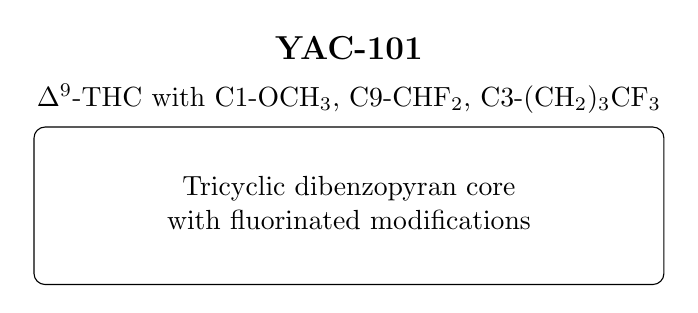
\begin{tikzpicture}[scale=0.8]
\node at (0,0) {\large\textbf{YAC-101}};
\node at (0,-0.8) {$\Delta^9$-THC with C1-OCH$_3$, C9-CHF$_2$, C3-(CH$_2$)$_3$CF$_3$};
\node[draw, rounded corners, minimum width=8cm, minimum height=2cm] at (0,-2.5) {
\begin{tabular}{c}
Tricyclic dibenzopyran core \\
with fluorinated modifications
\end{tabular}
};
\end{tikzpicture}
\end{center}

\subsection{YAC-201 Prodrug Activation}

\begin{center}
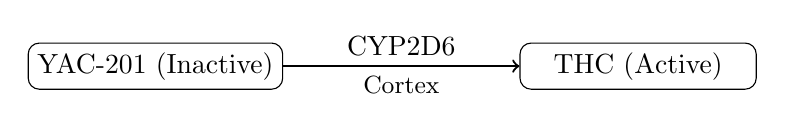
\begin{tikzpicture}[node distance=2cm, auto]
\node[draw, rounded corners, minimum width=3cm] (prodrug) {YAC-201 (Inactive)};
\node[draw, rounded corners, minimum width=3cm, right=3cm of prodrug] (active) {THC (Active)};
\draw[->, thick] (prodrug) -- node[above] {CYP2D6} node[below] {\small Cortex} (active);
\end{tikzpicture}
\end{center}

\end{document}
